\documentclass[
	a4paper,     		%% Papiergroesse: A4 OBSOLETE
%	twoside,     		%% Zweiseitiges Layout (alternativ: oneside)
	headsepline, 		%% Horizontale Linie unter Kopfzeile
	footsepline, 		%% Horizontale Linie ueber Fusszeile
	titlepage,   		%% Eigenstaendige Titelseite (alternativ: notitlepage)
%	halfparskip, 		%% Halbe Leerzeile zwischen zwei Abschnitten (alternativ: parskip, ...)
	12pt,        		%% Schriftgroesse: 12pt (alternativ: 10pt, 11pt, ...) OBSOLETE
%	bibtotoc,			%% Bilbiographie in's Inhaltsverzeichnis aufnehmen
%	liststotoc,			%% Indexe in's Inhaltsverzeichnis aufnehmen
%	smallheadings,		%% Kleine Ueberschriften
%	DIV1,				%% Divisor, Zeilenl�nge ca. 70 Zeichen
%	BCOR01cm,			%% Bindekorrektur
%	draft			  	%% Entwurfsmodus, volle/leere Boxen markieren
%	abstracton			%% Titel "`Zusammenfassung"' einschalten
]{scrreprt}

%%%
%%% Pakete
%%%

%%% Literaturverzeichnis, deutschen Stil benutzen (dinat)
%%% TODO: funktioniert leider derzeit nicht mit TeXlipse!
\usepackage[square]{natbib}
% \citestyle{dinat}

%%% Grafik
\usepackage{pstricks}

%%% Subfigures
\usepackage{subfig}

%%% Deutsche Sprache verwenden
\usepackage{ngerman}

%%% Kodierung der Eingabezeichen setzen (fuer dt. Umlaute etc.)
%%% Für Linux: [latin1] für Windows: [ansinew]
\usepackage[utf8]{inputenc}

%%% Zeichen-Kodierung in PDF-Dokumenten
\usepackage[T1]{fontenc}
%\usepackage{ae,aecompl}

%%% Web-Addressen auch mit T1-Encoding
\usepackage[T1]{url}
%%% ... und in tt-Font
\urlstyle{tt}

%%% amsmath, amssymb, amstext: Unterstuetzung div. mathematischer Zeichen etc.
\usepackage{amsmath,amssymb,amstext}

%%% PostScript-Fonts ersetzen
\usepackage{psfrag}

%%% Programmcode einbinden, Listings
\usepackage{listings}

%%% Farb-Unterstuetzung
\usepackage{color}

%%% Tabellen
\usepackage{booktabs}
\usepackage{array}
\usepackage{multirow}
\usepackage{tabularx}
\usepackage{threeparttable}	% Fussnoten in table-Umgebung

%%% Floats strikter positionieren (Option 'H'ere)
\usepackage{float}

%%%
%%% Pakete konfigurieren, Definitionen
%%%

%%% Ueberschriften bis zur Ebene 3 nummerieren
\setcounter{secnumdepth}{3}
\setcounter{tocdepth}{3}

%%% Neue Spaltentypen definieren
\newcolumntype{N}{>{\bfseries\scriptsize}l}
\newcolumntype{V}[1]{
	>{\bfseries\scriptsize\raggedright\hspace{0pt}}p{#1}
}

%%%
%%% Seitenlayout, Schriften
%%%

%%% scrpage2: KOMA Kopf- und Fusszeile
\usepackage[automark]{scrpage2}

%%% KOMA-Script: Optionen
% \KOMAoptions{fontsize=12pt}
% \KOMAoptions{paper=a4}

%%% EM unterstrichen darstellen
%\usepackage{ulem}

%%% Schrift fuer Captions verkleinern
\setkomafont{captionlabel}{\scriptsize}
\setkomafont{caption}{\usekomafont{captionlabel}}

%%% Schrift fuer Ueberschriften umstellen
%\setkomafont{sectioning}{\normalcolor\bfseries}

%%% Schriften fuer Titel- und Fusszeile umstellen
%\setkomafont{pagehead}{\normalfont\sffamily}
\setkomafont{pagenumber}{\normalfont\rmfamily\slshape}

%%% Unterstuetzung fuer Grafiken
\usepackage[dvips]{graphicx}
\DeclareGraphicsExtensions{.eps}
\graphicspath{{../images}}

%%% Hyperlinks in PS-Dokumenten, Optionen s.o.
\usepackage[%
  dvips,%
  colorlinks=false,%
  breaklinks=true,%
]{hyperref}

%%% Informationen ueber das PDF-Dokument setzen
\hypersetup{
  pdftitle={Zielsetzung und Vorgehensweise bei der Einführung eines QMS auf 
  Basis ISO 9001:2000},%
  pdfauthor={Jan Tammen (jan.tammen@htwg-konstanz.de)},%
  pdfsubject={Qualitätssicherung und Produkthaftung},%
  pdfcreator={Jan Tammen (jan.tammen@htwg-konstanz.de)},%
  pdfkeywords={Qualitätssicherung, QMS, ISO 9001:2000},
  pdfproducer={\LaTeX\ with package \flqq hyperref\frqq}, %%
%   colorlinks=true,
%  linkcolor=Gray,
%  urlcolor=Gray,
  bookmarksopen=true,
  pdfpagemode=UseOutlines,
  pdfview=FitV, % FitH
  pdfstartview=FitV,
  pdfhighlight=/I,
%   pdfborder=0 0 0, % keine Box um die Links!
  bookmarksnumbered=false,
  plainpages=false,
}

%%% Links im dvips-Mode auch umbrechen
%\usepackage{breakurl}

%%%
%%% Layout der Titelseite
%%%

%%% Titelkopf, erscheint oberhalb des Titels
\titlehead{
	\begin{figure}[H]
		\centering
		
\includegraphics[width=\textwidth]{../images/htwg-logo}
	\end{figure}
}

%%%% Subject, erscheint oberhalb des Titels
\subject{Qualitätssicherung und Produkthaftung, SS 07}

%%% Titel
\title{Zielsetzung und Vorgehensweise bei der Einführung eines QMS auf Basis ISO
9001:2000}


%%% Publisher, hier: Verantwortlicher Prof.
\publishers{%
	\small
  Bernd Wiedenroth, Fakultät Informatik, HTWG Konstanz
}

%%%% Autor. Weitere Autoren mit \and{<Name>} hinzufuegen
\author{%
  Jan Tammen (Matrikel-Nr. 277143)
}%

%%% Datum setzen
\date{\today}

%%% Rueckseite der Titelseite
% \lowertitleback{%
% 	\footnotesize%
% 	Erstellt mit \LaTeXe\ unter Verwendung des \KOMAScript-Pakets.
% }

%%%
%%% Header und Footer
%%%

\pagestyle{scrheadings}

%%% Kopfzeile in den Rand ragen lassen
%\setheadwidth{textwithmarginpar}

%%% Fusszeile in den Rand ragen lassen
%\setfootwidth{head}

%%% \automark[rechte Seite]{linke Seite}
%\automark[subsection]{section}

%% Header links -- section
%\ihead[]{\rightmark}

%% Header rechts -- chapter
%\ohead[]{\leftmark}

%% Header mittig -- leer
\chead[]{}

%% Footer mittig -- leer
\cfoot[]{}

%% Footer rechts -- Seitenzahl
\ofoot[]{\thepage}

%%% Footer links -- Titel der Arbeit
\ifoot[]{\footnotesize{Hausarbeit QUAS SS 07}}

%%%
%%% Sonstiges
%%%

%%%
%%% Beginn Hauptdokument
%%%
\begin{document}

%%% Titelseite erstellen
\maketitle

%%% Inhaltsverzeichnis erstellen
%\newpage
\tableofcontents

%%%
%%% Beginn Inhalt
%%%
\chapter{Einleitung}
\section{The Mozart Programming System}
In der vorliegenden Ausarbeitung soll das "`Mozart Programming System"'
\footnote{\url{http://www.mozart-oz.org}} 
vorgestellt werden. Bei \textsl{Mozart} handelt es sich um eine 
Programmierumgebung, die die multiparadigmische Programmiersprache \textsl{Oz} 
implementiert.

Entstanden ist Mozart-Oz ursprünglich als Forschungsprojekt am Deutschen 
Forschungszentrum für Künstliche Intelligenz (DFKI) sowie der Universität 
Saarbrücken. Inzwischen wird die Sprache vom Mozart-Konsortium, zu welchem 
Arbeitsgruppen aus Belgien, Schweden und Deutschland gehören, weiterentwickelt. 
Die Quellen sind unter einer Open-Source-Lizenz verfügbar; ein kommerzieller 
Einsatz der Sprache ist ebenfalls möglich.

Ähnlich wie in Java können Oz-Programme in eine Art Byte-Code übersetzt werden 
und laufen anschließend in einer virtuellen Maschine ab. Auf diese Weise wird 
eine gewisse Plattformunabhängigkeit erreicht.

\section{Die Programmiersprache Oz}
\subsection{Features}
Als Hauptfeatures und -vorteile von Oz gelten die folgenden Aspekte:

\begin{description}
  \item[Nebenläufigkeit] Arbeit mit leichtgewichtigen Threads, 
  Datenfluss-Synchronisation.
  \item[Inferencing] Constraintbasierte und 
  logische Programmierung.
  \item[Verteilung] Transparente 
  Netzwerkunterstützung.
  \item[Flexibilität] Dynamische Typisierung, inkrementelles 
  Kompilieren.
\end{description}

\subsection{Datentypen}
Die Sprache stellt eine Reihe von Datentypen zur Verfügung, deren Hierarchie in 
Abbildung \ref{fig:oz-datentypen} dargestellt ist.

\begin{figure}[hp]
  \centering 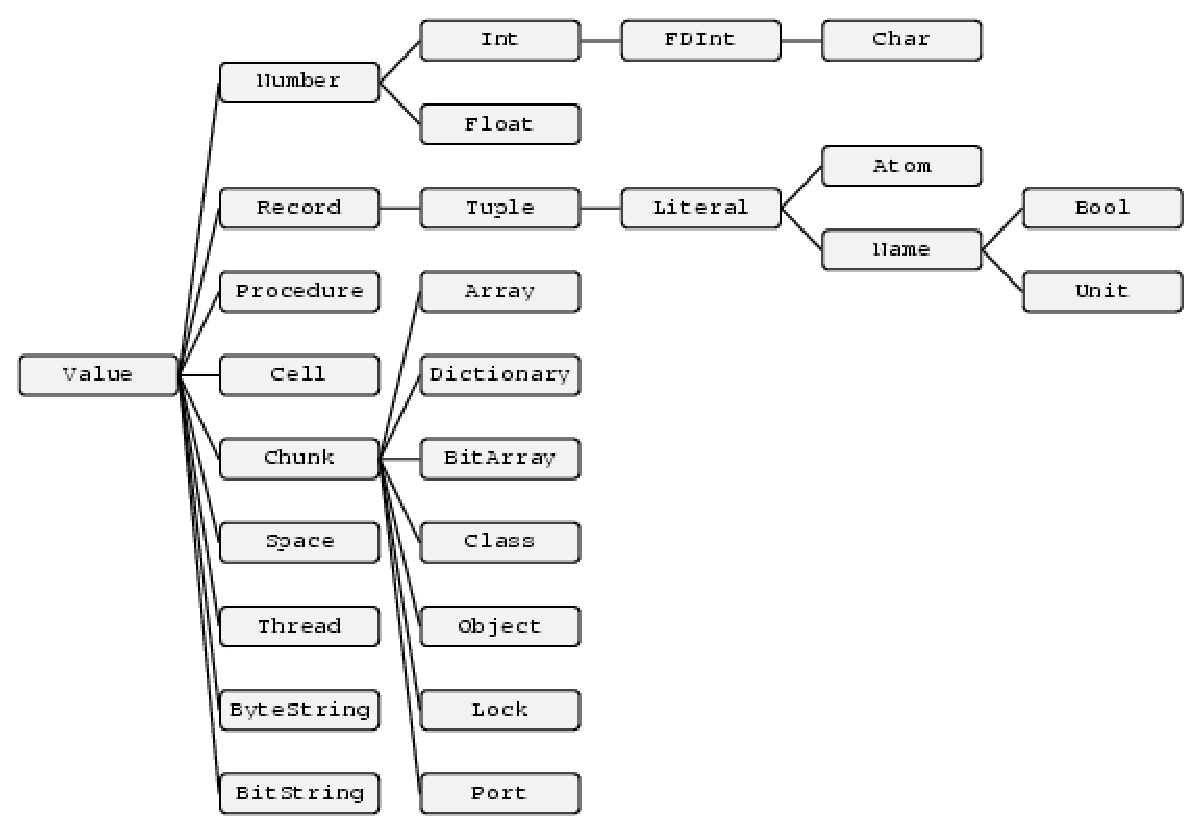
\includegraphics[width=0.70\textwidth]{../images/oz-datentypen} 
  \caption{Hierarchie der Datentypen in Oz 3. Quelle:
  \cite[Tutorial of Oz, Chapter 3.1]{url:mozart-documentation}}
  \label{fig:oz-datentypen}
\end{figure}

Einige der wichtigsten Datentypen seien hier kurz aufgeführt (vgl. 
\cite{Brunklaus:00}).

\begin{enumerate}
  \item Einfache Werte
    \begin{description}
      \item [Zahlen] können in Oz sowohl als ganze Zahlen (\texttt{Int, Char})
      als auch Fließkommazahlen (\texttt{Float}) benutzt werden.
      \item[Literale] teilen sich auf in sog. Atome und Namen. Ein Atom wird 
      durch eine alphanumerische Zeichenkette beschrieben, die entweder mit 
      einem Kleinbuchstaben beginnt oder in Hochkomma gefasst ist. Namen sind 
      eindeutige Bezeichner, die über eine spezielle Prozedur namens 
      \texttt{NewName} erzeugt werden können.
      \item[Prozeduren] können in Oz an Variablen gebunden und auch zur 
      Laufzeit erzeugt werden. \end{description}
  \item Zusammengesetzte Werte
    \begin{description}
      \item[Records] bestehen aus einem Bezeichner (Label) sowie einer festen 
      Anzahl von Komponenten oder Argumenten. Argumente bestehen aus dem Tupel 
      (Feature, Feld).
      \item[Tupel] sind ein Spezialfall von Records, bei denen die Argumente 
      kein explizites Feature besitzen.
      \item[Listen] sind eine Sonderform der Tupel. Die leere Liste wird mit
      \texttt{nil} denotiert, offene Listen bspw. als \texttt{1|2|3|nil} und 
      geschlossene Listen (also Listen mit fester Elementanzahl) als \texttt{[1 
      2 3]}.
    \end{description}
  \item \textbf{Chunks} erlauben es, abstrakte Datentypen zu konstruieren. 
  Oz bringt bereits einige vordefinierte Chunks mit, z.B. \texttt{Array} 
  oder \texttt{Dictionary}.
\end{enumerate}

\subsection{Multiparadigmisch?}
Wie bereits eingangs erwähnt, unterstützt Oz mehrere Programmierparadigmen:

\begin{enumerate}
  \item Constraint-Programmierung
  \item Funktionale Programmierung
  \item Objektorientierte Programmierung
  \item Logische Programmierung
\end{enumerate}
  
Im Gegensatz zu einer Programmiersprache, die nur eines der Paradigmen 
unterstützt, lassen sich in Oz also die zu lösenden Probleme von mehreren 
Seiten gleichzeitig mit dem jeweils geeignetsten Paradigma bearbeiten. 
Erreichen könnte man dies zwar auch durch die Kombination verschiedener 
Programmiersprachen, dabei bliebe aber der Nachteil, dass man semantische 
Lücken überwinden und Schnittstellen zwischen den einzelnen Sprachen definieren 
müsste. Dies würde u.a. zu einer aufwendigeren Fehlersuche führen. Mit Oz 
lassen sich hingegen die verschiedene Paradigmen problemlos miteinander 
kombinieren, deren gemeinsame Basis, das Oz Programming Model, im nächsten 
Abschnitt vorgestellt wird.

\subsection{Programmiermodell (Oz Programming Model, OPM)}
Die Grundlage für Berechnungen in Oz bildet das so genannte \textsl{Concurrent 
Constraint Programming}. Alle weiteren Paradigmen werden durch sog. "`syntactic 
sugar"' (Syntaxerweiterungen) in die Sprache integriert \cite{KI-LP96}.

Allgemein verwendet das Modell für Berechnungen die Metapher eines sog. 
\textsl{Berechnungsraums} (Computational Space). In diesem befindet sich zum 
einen ein \textsl{Speicher}, zum anderen eine Anzahl von sog. \textsl{Aktoren}. 
Aktoren führen die eigentlich Berechnung durch, indem sie schrittweise 
reduziert werden und sich dabei über den gemeinsamen Speicher synchronisieren. 
Dazu können Aktoren Information in den Speicher schreiben (tell) und auf 
Information warten und diese anfordern (ask).

Nebenläufigkeit (Concurrency) ist einer der wichtigsten Aspekte des OPM. Dabei 
bedeutet Nebenläufigkeit, dass verschiedene Berechnungen unabhängig voneinander 
durchgeführt werden können, nicht, dass diese parallel ablaufen.


\chapter{Das Beispiel-Unternehmen}
Als Beispiel soll in dieser Ausarbeitung die fiktive Software-Firma 
\emph{foobar GmbH} dienen. Es handelt sich dabei um eine mittelständische Forma 
mit 20 Angestellten. Zu ihren Kunden gehören hauptsächlich mittelgroße und große
Verlage, Versicherungen und Banken. Für diese Kunden werden
Individualsoftwaresysteme konzipiert, erstellt und betreut.

Die Struktur des Unternehmens lässt sich wie folgt in mehrere Bereiche
aufteilen: 

\begin{description}
  \item[Marketing und Vertrieb:] 2 Mitarbeiter. Diese Abteilung ist
  verantwortlich für die Darstellung des Unternehmens nach außen sowie die
  Akquise neuer sowie Betreuung bestehender Kunden. So werden z.B. Werbe- oder
  Stellenanzeigen geschaltet und Messebesuche durchgeführt.
  \item[Entwicklung:] 14 Mitarbeiter. Die größte Abteilung der Firma kümmert
  sich um das Design und die Entwicklung der Kundenprojekte. Das Entwicklerteam
  besteht dabei komplett aus Hochschulabsolventen und es arbeiten Mitarbeiter
  unterschiedlicher Erfahrungsgrade zusammen. Die Entwicklungsabteilung ist
  aufgeteilt auf 2 Projektteams, die wiederum durch jeweils einen Projektleiter
  nach außen hin vertreten werden.
  \item[Support:] 2 Mitarbeiter. In dieser Abteilung werden alle dringenden
  Kundenanfragen entgegengenommen und bearbeitet. Sofern es sich nicht um
  allgemein lösbare Probleme handelt, werden diese je nach Schweregrad sofort an
  das zuständige Entwicklerteam weitergeleitet.
  \item[Verwaltung:] 1 Mitarbeiter. Zu den Aufgaben dieser Abteilung gehört die
  Terminverwaltung, Bestellung von Bürdobedarf sowie die Buchhaltung.
\end{description}

Da es sich bei den Kunden teils um Unternehmen aus der Finanzwirtschaft 
handelt, bestehen natürlich erhöhte Anforderungen an die Qualität der von der 
Firma erstellten Produkte.

\chapter{Einführung eines Qualitätsmanagementsystems}
\section{Zielsetzungen} \label{sec:ziele}
Je nach Art und Größe des Unternehmens stehen bei der Einführung eines QMS 
unterschiedliche Zielsetzungen im Vordergrund. Ist für manche Firmen der reine 
Erwerb eines QMS-Zertifikats das Hauptziel, um damit - vermeintlich - höhere 
Markchancen zu erlangen, so kann der Einsatz eines funktionierenden QMS 
tatsächlich einen Mehrwert für die Firma bedeuten. Denn durch eine konsequente 
Umsetzung lassen sich die unternehmensinternen Abläufe optimieren und letztlich 
die Mitarbeiter- sowie Kundenzufriedenheit erhöhen. Wird eine Zertifizierung 
nur zum Selbstzweck angestrebt, so werden die Vorgaben eines QMS stur umgesetzt 
und abgearbeitet, sodass am Ende eher eine Verschlechterung der Effizienz und 
verärgerte bzw. uninformierte Mitarbeiter stehen.

Zu den Zielsetzungen können u.a. die folgenden Punkte gehören:

\begin{itemize}
  \item Rechtliche Aspekte: Rechtssicherheit und Nachweissicherheit,
  \item Wirtschaftliche Aspekte: Reduktion der Fehlerkosten,
  \item Marktaspekte: Verbesserung des Images, Vorteile gegenbüber 
  Wettbewerbern,
  \item Qualitätsaspekte: Erhöhung der Produktqualität, Umsetzung einer 
  Qualitätsstrategie,
  \item Firmeninterne Aspekte: Erhöhung der Transperanz betrieblicher Abläufe
  und der Mitarbeitermotivation.
\end{itemize}

Das meiner Einschätzung nach wichtigste Ziel bei der Einführung eines QMS ist 
jedoch \emph{die Erhöhung der Kundenzufriedenheit} durch bessere Erfüllung der 
Kundenanforderungen. In den folgenden Abschnitten möchte ich auf die einzelnen
Zielsetzungen detaillierter eingehen.

\subsection{Rechtliche Aspekte}
Die Kundenstruktur des Unternehmens erfordert es, dass die Produkte erhöhten
Qualitätsansprüchen genügen, da von den Kunden u.a. finanzkritische
Applikationen betrieben werden. Durch den Einsatz eines QMS will man dem Kunden
nach außen hin zeigen, dass das Thema Qualität ernstgenommen wird und ein
definierte Systematik angewandt wird. 

\subsection{Marktaspekte}
Im Bereich der Software-Entwicklung sieht die \emph{foobar GmbH} derzeit keine
besonderen Vorteile durch eine Zertifizierung. Jedoch kann mit einem derartigen
Zertifikat geworben werden und man verschafft sich einen Vorteil gegenüber
Mitbewerbern. Einige der Kunden des Unternehmens sind Banken, und in Zukunft
verlangen diese eine Zertifizierung von allen Software-Lieferanten. Vor diesem
Hintergrund ist die Einführung eines (zertifizierten) QMS überlebenswichtig für
das Unternehmen, um nicht Kunden zu verlieren.

\subsection{Qualitätsaspekte}
Als Dienstleistungsunternehmen steht für unsere Beispielfirma die
Kundenzufriedenheit an oberster Stelle. Die an den Kunden ausgelieferte Software
sollte möglichst fehlerfrei, gut getestet und dokumentiert sein. Auf etwaige
auftretende Probleme muss schnell reagiert werden können, damit dem Kunden durch
Ausfälle kein Schaden entsteht.

Die Qualität der Software soll konkret durch die Einführung regelmäßiger Code-
und Projekt-Reviews, Mitarbeiter-Schulungen sowie entsprechende Vorgehensmodelle
und Hilfswerkzeuge bei der Entwicklung erhöht werden. Als Nebeneffekt erhofft
man sich durch diese Maßnahmen auch eine Erhöhung der Mitarbeiterzufriedenheit,
da die Entwickler teilweise durch immer wiederkehrende Probleme und Fehler
unnötigen Belastungen ausgesetzt waren.

\subsection{Wirtschaftliche Aspekte}
Direkt im Zusammenhang mit der Qualität stehen die wirtschaftlichen Aspekte.
Denn durch mangelhafte Produkte entstehen dem Unternehmen direkte Kosten, die
für die Beseitigung der Fehler aufgewendet werden müssen. Durch die Erhöhung der
Qualität sollten demnach gleichzeitig die Kosten sinken. 

Weiterhin sollen die Personalkosten durch die Optimierung der Arbeitsabläufe
reduziert werden und z.B. alternative Entwicklungsmodelle (wie z.B. eXtreme
Programming) erprobt werden, durch welche die Effizienz der Mitarbeiter
gesteigert werden kann.

\subsection{Firmeninterne Aspekte}
Durch die Verbesserung der firmeninternen Abläufe soll zum einen die Transparenz
der Firmenstruktur erhöht werden. Entscheidungswege sollen möglichst kurz
gehalten werden, um wichtige Entscheidungen nicht unnötig zu verzögern.
Entwickler sollen wenn möglich im direkten Kontakt mit den Kunden stehen, um
nicht durch weitere Zwischenstationen eine unnötige Fehlerquelle einzufügen.

Durch diese Maßnahmen erhofft sich die \emph{foobar GmbH} u.a. eine gesteigerte
Motivation der Mitarbeiter, da diese direkter in die Entscheidungen der Firma
eingebunden sind und Veränderungen direkt sichtbar werden.

\section{Vorgehensweise}
Bei der Einführung eines QMS ist eine schrittweise Vorgehensweise sinnvoll. 
Abbildung \ref{fig:qms-schritte} zeigt diese auf.

\begin{figure} 
  \centering
  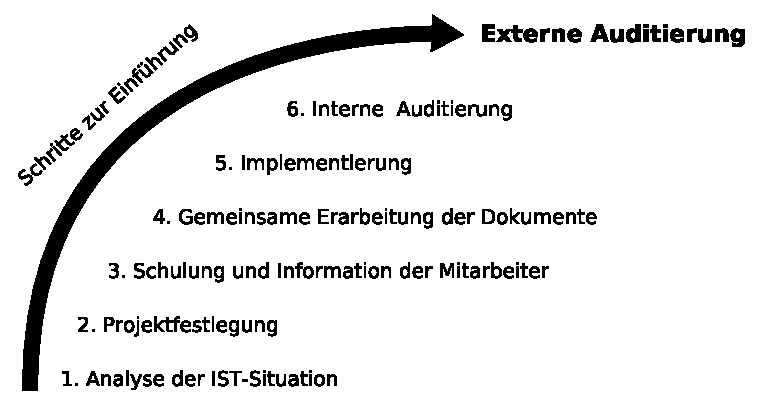
\includegraphics[width=0.8\textwidth]{../images/qms-schritte}
  \caption{Vorgehensweise bei der Umsetzung eines QM-Systems 
  \citep[vgl.][]{quas}.}
  \label{fig:qms-schritte}
\end{figure}

In den folgenden Abschnitten werden die einzelnen Schritte näher beschrieben.

\subsection{IST-Zustand-Analyse}
Die IST-Analyse dient dazu, die momentane Situation innerhalb der Organisation
zu erfassen und zu dokumentieren. Es werden dabei Erkenntnisse für
Verbesserungen, fehlende Verfahren, Mittel und Methoden festgehalten. In dieser
Phase entstehen erste Ansätze für mögliche Verbesserungen und das weitere
Vorgehen \citep{url:zert}.

Zur Analyse der bestehenden Prozesse bietet es sich an, auf die Dienste eines
externen Dienstleisters zurückzugreifen. Zu den Kernprozessen der Firma
\emph{foobar GmbH} gehören u.a.:

\begin{itemize}
  \item Analyse und Design einer Software-Anwendung,
  \item Implementierung einer Software-Anwendung,
  \item Bearbeitung von Support-Anfragen.
\end{itemize}

Als weitere Unterstützung zur Erstellung der IST-Analyse kann der in
der DIN EN ISO 9001:2000 enthaltene Fragenkatlog herangezogen werden.

\subsection{Projektfestlegung}
Ziel dieser Phase ist es, einen Projektplan zu erstellen, der den weiteren
Verlauf der Maßnahmen aufzeigt. Inhalt des Projektplans sollte u.a. sein:

\begin{itemize}
  \item Liste der zu erarbeitenden Dokumente und dafür verantwortliche
  Mitarbeiter,
  \item Zeitrahmen für die Erstellung der Dokumente,
  \item erwarteter Umfang der Dokumente.
\end{itemize}

Weiterhin sollte der Projektplan Meilensteine enthalten, mit deren Hilfe der 
Vorgang besser kontrolliert werden kann. Die Firma \emph{foobar Gmbh} 
beauftragt ein externes Beratungsunternehmen mit der Erstellung des 
Projektplans, welcher sich auf die in Kapitel \ref{sec:ziele} beschriebenen 
Zielsetzungen stützt \citep{wittmeier}.

\subsection{Schulung und Information der Mitarbeiter}
Die Inhalte des erstellten Projektplans müssen an die Mitarbeiter kommuniziert
werden, um sie aktiv in den Prozess einzubinden. Auch müssen ihnen die
Zielsetzungen für die Einführung des QMS aufgezeigt werden, damit bei der
Umsetzung alle an einem Strang ziehen können.
Die Mitarbeiter der Firma werden in einigen durch die Geschäftsführer gehaltenen
Vorträgen über das Vorhaben informiert und erhalten die Gelegenheit, ihre
Bedenken und Vorschläge einzubringen. Dadurch entstehen u.U. wertvolle
Änderungen am Projektplan, wodurch sich die Mitarbeiter noch besser in die
Firmenpolitik mit einbezogen fühlen.

\subsection{Gemeinsame Erarbeitung der Dokumente}
Wo dies möglich ist, sollten die Angestellten in die Erarbeitung der
im Projektplan geforderten Dokumente einbezogen werden. Dadurch wird
die Identifikation mit den anstehenden Änderungen und Maßnahmen erhöht. Man
hofft dadurch, dass womöglich unangenehme Veränderungen so besser durch das
Personal angenommen werden. Die in dieser Phase erzeugten Dokumente dienen
vorwiegend folgenden Zwecken:

\begin{itemize}
  \item Erleichterung der Einweisung/Einarbeitung neuer Mitarbeiter,
  \item Darstellung des Unternehmens und seiner Qualitätsfähigkeiten nach außen 
  (QM-Handbuch),
  \item Nachschlagewerk für seltenere oder schwierigere Tätigkeiten.
\end{itemize}

Das QM-Handbuch beschreibt alle Elemente der ISO und ist in mehrere Abschnitte 
gegliedert. Es werden die Organisation und die betrieblichen Abläufe 
dokumentiert. Das Handbuch dient dabei auch als Aushängeschild des Unternehmens 
und kann von Kunden eingesehen werden. Die Dokumentation wird dabei wiederum 
zusammen mit den zuständigen Mitarbeitern erstellt. Für alle 
qualitätsrelevanten Aspekte werden Verantwortlichkeiten verteilt und 
festgehalten. Außerdem werden in dieser Phase Verfahrens- und 
Arbeitsanweisungen, Auditberichte, Qualitätsberichte, Ergebnisberichte und 
Protokolle erstellt \citep{quas}.

\subsection{Implementierung}
In dieser Phase sollen die erarbeiteten Konzepte mithilfe der Mitarbeiter in 
Maßnahmen umgesetzt werden. Dabei geht es u.a. darum, die im Maßnahmenkatalog 
festgehaltenen Fehlerquellen zu vermeiden sowie Aufbau- und 
Ablauforganisationen zu optimieren. Allgemein sollte eine Verbesserung der 
Prozessabläufe erreicht werden. Eine schrittweise Einführung und Vorstellung der
neuen Abläufe ist zweckmäßig, um die Angestellten nicht mit zu abrupten
Veränderungen zu überfordern. Im Beispiel der Firma \emph{foobar GmbH} sollen
Supportanfragen zukünftig nicht mehr unnötig lange durch die Support-Abteilung
bearbeitet werden, sondern sofort an die zuständigen Entwickler weitergegeben
werden. 

Sollten sich einzelne Prozessabläufe mit der Zeit ändern oder die im 
Maßnahmenkatalog definierten Änderungen nicht den gewünschten Effekt gebracht 
haben, kann es notwendig sein, die Prozessabläufe und die zuvor erstellte 
Dokumentation anzupassen. Die ISO 9000 prägt hierzu den Begriff "`ständiger 
Verbesserungsprozess"', welcher in Abbildung \ref{fig:qm-prozess} dargestellt 
ist.

\subsection{Interne Auditierung}
Nach Einführung der geplanten QM-Maßnahmen muss durch interne Auditierungen
festgestellt werden, ob die eingeführten Maßnahmen auch entsprechend umgesetzt
wurden. Außerdem muss periodisch überprüft werden, ob die Maßnahmen noch
zweckhaft sind, oder evtl. gestrichen bzw. modifiziert werden. Da es sich bei
unserere Beispiel-Firma um ein kleines Unternehmen handelt, werden diese
Auditierungen direkt von den zwei Geschäftsführern durchgeführt, es gibt also
keinen dedizierten Qualitätsbeauftragten.

\section{Externe Auditierung}
Am Ende des Prozesses steht die externe Auditierung sowie die Zertifizierung
durch eine Zertifizierungsstelle - sofern dies vom Unternehmen gewünscht ist.
Die \emph{foobar GmbH} entscheidet sich dafür, ein entsprechend
akkreditiertes Zertifizierungsunternehmen zu beauftragen und das eingeführte
QM-System zu prüfen.


\chapter{Fazit}
Abschlie�end k�nnen wir feststellen, dass die \acr{xml}-Unterst�tzung der untersuchten \acr{dbms} sehr umfangreich ist und viele M�glichkeiten f�r die Verarbeitung von \acr{xml}-Daten bietet. Die f�r das Anwendungsbeispiel aufgestellten Anforderungen konnten mit allen drei \acr{dbms} umgesetzt werden.

Auf der anderen Seite ist die breite Unterst�tzung von \acr{xml}-Funktionalit�ten auch ein Nachteil, da sich der Einarbeitungsaufwand dadurch erh�ht. Bei den "`\acr{xml}-enabled"' Datenbanken steigert sich die Komplexit�t der Anfragen durch Benutzung der \acr{xml}-Funktionen erwartungsgem��.

Die Umsetzung des \acr{sql}/\acr{xml}-Standards ist sowohl bei Oracle 9i wie auch beim SQL-Server 2005 nicht vollst�ndig, wobei Oracle sich wesentlich n�her am Standard orientiert. XPath und XQuery sind beim SQL-Server und eXist vollst�ndiger umgesetzt als bei Oracle. 

Unserer Ansicht nach war der gr��te Nachteil bei der Umsetzung der Anwendung, dass bisher keine Modellierungssprache bei der Verwendung von \acr{xml} existiert. Folglich wird ein strukturiertes Vorgehen bei der Analyse deutlich erschwert. Dieses Problem tritt besonders bei der hybriden Speicherung von \acr{xml}-Daten auf. Wir haben das Problem dadurch umgangen, indem wir uns am bestehenden relationalen Datenmodell orientiert haben.

In unserem Fallbeispiel wurden durch die Benutzung von \acr{xml} keine M�glichkeiten geschaffen, die nicht auch durch die Benutzung von rein relationalen Daten bestanden h�tten. Vorteile h�tten sich ergeben, wenn ein Datenaustausch zwischen den \acr{dbms} existiert h�tte. Beispielsweise wenn die Wohnungsdaten bereits in \acr{xml} vorgelegen h�tten oder ein \acr{xml}-Export der Rechnungsdaten n�tig gewesen w�ren.

%%%
%%% Anhaenge: Glossar, Bibliographie...
%%%

%%% Bibliographie-Stil
% abbrvdin, alphadin, plaindin, unsrtdin
\bibliographystyle{dinat}

%%% Anstatt 'Literatur' -> 'Quellen'
\renewcommand{\bibname}{Quellen}

%%% Bibliographie ausgeben
\bibliography{Quellen}

%%% Glossar ausgeben
%\printgloss{Glossar}

\end{document}